\documentclass[a4paper,12pt,abstract=on,twoside,openright,parskip=full]{book}
\setlength\parindent{1.5em}
\setlength{\parskip}{1.3ex plus 0.5ex minus 0.3ex}

\usepackage[todo]{../general}

\hypersetup{pdfauthor={André Martins Pereira}}
\hypersetup{pdftitle={Pre-Thesis: Efficient processing of ATLAS events analysis in platforms with accelerator devices}}

\bibliography{../bib/refs}
\graphicspath{{../imgs/}{../charts/}}

% reduce chapter margins
%\renewcommand{\chapterheadstartvskip}{\vspace*{-1.6\baselineskip}}

\begin{document}
\pdfbookmark{Cover}{cover}
\pagenumbering{roman}

%titlepage
\thispagestyle{empty}
\begin{center}
\begin{minipage}{0.75\linewidth}
    \centering
%University logo
    
\includegraphics[scale=1]{imgs/logo.png}
    \par
    \vspace{3cm}
%Thesis title
    {\uppercase{\Large An efficient particle physics data analysis framework for homogeneous and heterogeneous platforms\par}}
    \vspace{3cm}
%Author's name
    {\large André Pereira\\\texttt{ampereira@di.uminho.pt}\par}
    \vspace{3cm}
%Degree
    {\Large A pre-thesis submitted for the degree of Doctor of Philosophy\par}
    \vspace{3cm}
%Date
    {\Large July 2014}
\end{minipage}
\end{center}
\clearpage

\pagestyle{fancy}
\renewcommand{\headrulewidth}{0.4pt}
\fancyhead[LO,RE]{}
\fancyhead[LE]{\slshape \leftmark}
\fancyhead[RO]{\slshape \rightmark}
\fancyfoot[RO,LE]{\thepage}%
\fancyfoot[C]{}

\fancypagestyle{plain}{%
  \renewcommand{\headrulewidth}{0.0pt}
  \fancyhead{}
  \fancyfoot[C]{}
  \fancyfoot[RO,LE]{\thepage}
}

\pagenumbering{arabic}

\tableofcontents


%
% include all tex/ chapter files
%

%!TEX root = ../main.tex

\chapter{Introduction}
\label{introduction}

Today's computing platforms are becoming increasingly complex with multiple interconnected computing nodes, each with multiple multicore CPU chips, and sometimes coupled with hardware accelerators. While the application performance is an important issue to tackle, the efficient usage of the resources of these systems is a crucial subject that needs to be addressed. Guaranteeing that the available computational resources are being adequately used by an application may require deep knowledge of the underlying architecture details of both CPUs and hardware accelerators, as well as extensive tuning of each individual application. It is crucial to comprehend the key issues that currently have more impact on computing performance and efficiency, namely the relationship between the cost of numerical computation, memory access, and data communication among available computing units. The architecture design of many-core hardware accelerators is significantly different among devices, with no standard yet defined. The programmer must know the architectural details of each hardware accelerator and their interconnection topology to the CPU to produce efficient code.

From the hardware point of view, efficiency may have a different meaning: it can be considered as the ratio between power usage and computational throughput. This is a subject of extensive research in a field also known as ``Green Computing'', where the goal is to reduce power consumption of the hardware while minimising the performance degradation. This is important for both mobile computing and to reduce the cost of maintaining huge computing clusters and data centres.

Computing clusters are the most popular High Performance Computing (HPC) platforms, constituted of many different computing nodes, interconnected by specialised communication channels in a distributed memory environment. The computing nodes may be characterised as homogeneous or heterogeneous platforms, where the former has one or more CPUs in a shared memory environment, and the latter has hardware accelerators coupled to the CPUs by a PCI-Express interface, in a distributed memory environment. This implies that the data is always visible to the CPUs, but must be explicitly transferred to the accelerator devices.

A proper data management is relevant to ensure the efficiency of an application. Code parallelism is a must to take advantage of the multiple cores in both the CPUs and the hardware accelerators, adapted to the different memory and programming paradigms. Data races, resource contention and, when considering heterogeneous platforms, explicit memory transfers are complex challenges for the programmer. Also, each accelerator manufacturer uses their own frameworks and compilers to program their devices. Non-computer scientists opt to invest most of the research time on their field of science and have little time to improve their programming skills. These factors reinforced the collaboration of multidisciplinary teams of scientists from various fields with computer scientists to develop high performing, efficient, and robust applications.

\section{Context}
\label{context}

The European Organization for Nuclear Research \cite{CERN} (CERN, acronym for \textit{Conseil Européen pour la Recherche Nucléaire}) is a consortium of 21 European countries and more than 30 ``observer'' countries, with the purpose of operating the largest particle physics laboratory in the world. Founded in 1954, CERN is located in the border between France and Switzerland, and employs thousands of scientists and engineers representing 608 universities and research groups of 113 different nationalities.

CERN research focus on the basic constituents of matter to understand the fundamental structure of the universe, which started by studying the atomic nucleus but quickly progressed into high energy physics (HEP), namely on the interactions between particles. The instrumentation used in nuclear and particle physics research is essentially formed by particle accelerators and detectors, alongside with the facilities necessary for delivering the protons to the accelerators. The Large Hadron Collider (LHC) particle accelerator (later presented) speeds up groups of particles close to the speed of light, in opposite directions, inducing a controlled collision at the detectors core (the collision of two particles is referred as an ``event''). The detectors record various characteristics of the resultant particles of each collision, such as energy and momentum, which originate from complex decay processes of the original particles. The purpose of these experiments is to test models and predictions in High Energy Physics (HEP), such as the Standard Model, by confirming or discovering new particles and interactions.

CERN started with a small low energy particle accelerator, the Proton Synchrotron \cite{CERN:PS} inaugurated in 1959, but soon its equipment was iteratively upgraded and expanded. The current facilities are constituted by the older accelerators (some already decommissioned) and particle detectors, as well as the newer Large Hadron Collider (LHC) \cite{CERN:LHC} high energy particle accelerator, located 100 meter underground and with a 27 km circumference length. There are currently seven experiments running on the LHC: CMS \cite{CERN:CMS}, ATLAS \cite{CERN:ATLAS}, LHCb \cite{CERN:LHCb}, MoEDAL \cite{CERN:MoEDAL}, TOTEM \cite{CERN:TOTEM}, LHC-forward \cite{CERN:LHCf} and ALICE \cite{CERN:ALICE}. Each of these experiments have their own detector on the LHC and conduct HEP analysis, using distinct technologies and research approaches. One of the most relevant researches being conducted at CERN is the validation of the Standard Model and discovery of the Higgs boson theory. The ATLAS experiment, a key project at CERN, aims to study the properties of the recently discovered Higgs boson \cite{Higgs}, the search for new particles predicted by models of physics beyond the Standard Model like Susy, searches for new heavy gauge bosons and precision measurements where the top quark is of utmost importance. During the next year the LHC will be upgraded to increase its luminosity, e.g., the amount of energy of the accelerated particle beams.

Approximately 600 millions of collisions occur every second at the LHC. Particles produced in head-on proton collisions interact with the detectors of the ATLAS experiment, generating massive amounts of raw data as electric signals. It is estimated that all the detectors combined produce 25 petabytes of data per year \cite{CERN:DATA1,CERN:DATA2}. CERN does not have the financial resources to afford the computational power necessary to process all data from the detectors, which motivated the creation of the Worldwide LHC Computing Grid \cite{CERN:WLHCCG}, a distributed computing infrastructure that uses the resources of the scientific community for data processing. The grid is organized in a hierarchy divided in 4 tiers. Each tier is made by one or more computing centres and has a set of specific tasks and services to perform, such as store, filter, refine and analyse all the data gathered at the LHC.

The Tier-0 is the data centre located at CERN. It provides 20\% of the total grid computing capacity, and its goal is to store and reconstruct the raw data gathered at the detectors in the LHC, converting it into meaningful information, to be used by the remaining tiers. The data is received on a format designed for this reconstruction, with information about the event, detector and software diagnostics. The output of the reconstruction has two formats, the Event Summary Data (ESD) and the Analysis Object Data (AOD), each with different purposes, containing information of the reconstructed objects and calibration parameters, which can be used for early analysis. This tier distributes the raw data and the reconstructed output by the 11 Tier-1 computational centres, spread among the different member countries of CERN.

Tier-1 computational centres are responsible for storing a portion of the raw and reconstructed data and provide support to the grid. In this tier, the reconstructed data suffers more processing and refinement, to filter the relevant information and reduce its size, which is now in Derived Physics Data (DPD) format, to be then transferred to the Tier-2 computational centres. The size of the data for an event is reduced from 3 MB (raw) to 10 kB (DPD). This tier also stores the output of the simulations performed at Tier-2. The Tier-0 centre is connected to the 11 Tier-1 centres by high bandwidth optical fiber links, which form the LHC Optical Private Network.

There are roughly 140 Tier-2 computational centres spread around the world. Their main purpose is to perform both Monte-Carlo simulations and a portion of the events reconstructions, with the data received from the Tier-1 centres. The Tier-3 centres range from university clusters to desktop computers, and they are responsible for most events reconstruction and final data analysis. In the CERN terminology, an application that is designed to process a given amount of data to extract relevant physics information about events, which may support a specific HEP theory, is called an analysis.

The Laboratório de Instrumentação e Física Experimental de Partículas (LIP) \cite{LIP} is a portuguese scientific and technical association for research on experimental high energy physics and associated instrumentation. LIP has a strong collaboration with CERN as it was the first scientific organisation from Portugal that joined CERN, in 1986. It has laboratories in Lisbon, Coimbra and Minho and 170 people employed. LIP researchers have produced several applications for testing at ATLAS several HEP theoretical models that use Tier-2 and Tier-3 computational resources for data analysis. Most of the analysis applications use in-house developed skeleton libraries, such as the LipCbrAnalysis and LipMiniAnalysis.

There is the need to process more data, more accurately, in less time, which often leads to investments on larger computing clusters to improve the quality of the research results. However, most scientific code was not designed and/or developed for an efficient use of the available computational resources of modern platforms. If these applications were adequately designed (or tuned), the event analysis throughput could be massively increased. An efficient parallel application can significantly improve its performance at a much lower cost \cite{Msc:AMP}.

\section{Problem and Motivation}
\label{motivation}

With an increase in particle collisions and data being produced by the detectors at the LHC, research groups will need a larger budget to acquire and maintain the required computational resources to keep up with the analysis. Moreover, research groups working on the same experiment enforce positive competition to find and publish relevant results. The amount and quality of event processing has a direct impact on the research, meaning that groups with access to the most efficient computational resources become ahead of the competition.

Improving the accuracy of each event analysis benefits the quality of the physics properties being studied. Due to several intrinsic ATLAS experimental effects like energy and transverse momentum resolutions, the measured kinematic properties of particles produced in a collision may be shifted within a range of $\pm1\%$, implying an uncertainty that is propagated through the event analysis. It is possible to improve the reconstruction quality by varying the values measured by the detector within that range, but with a significant impact to the analysis execution time, leading to a trade-off between the event processing throughput and their reconstruction quality.

Scientists at LIP developed the LipCbrAnalysis skeleton library to aid the development of data analysis applications. It contains a set of physics utilities, such as specific classes and functions, and removes the need to code the input file reading, memory allocation of each event data, and output creation for every data analysis application. With this, the programmer may focus on the specifics of the required analysis, such as the filtering and reconstruction of events. An improved version was developed, LipMiniAnalysis, aiming to read a new type of input data files, and stripping the former skeleton of outdated features.

An efficiency study and optimisation of one of LIP production data analysis, also used as a case study for a background research on this issue, was presented in \cite{Msc:AMP,paperAMP}. It tackled the computational inefficiencies of the application on both homogeneous and heterogeneous platforms, and identified several limitations to performance scalability, specially when using hardware accelerators. The data analysis case study and the limitations identified with the LipMiniAnalysis skeleton are presented in a later section.

At the LHC, two proton beams are accelerated close to the speed of light in opposite directions, set to collide inside a specific particle detector. This head-on collision triggers a chain reaction of decaying particles, and most of the final particles interact with the detector, allowing to record relevant data. One of the searches being conducted at the ATLAS Experiment relates to the study of the Higgs boson couplings to top quarks. Figure \ref{fig:ttH} represents the final state topology of the associated production of two top quarks and one Higgs boson (that decays to $b\bar{b}$, two bottom quarks), known as \ttH production. Figure \ref{fig:ttbar} provides a schematic representation of the system to highlight the key features, such as the bottom quarks being jets of smaller particles, and the leptons (both $l^+$ and $l^-$) being a muon and electron in the $t$ and $\bar{t}$ decays, respectively.

\begin{figure}[!htp]
	\begin{center}
		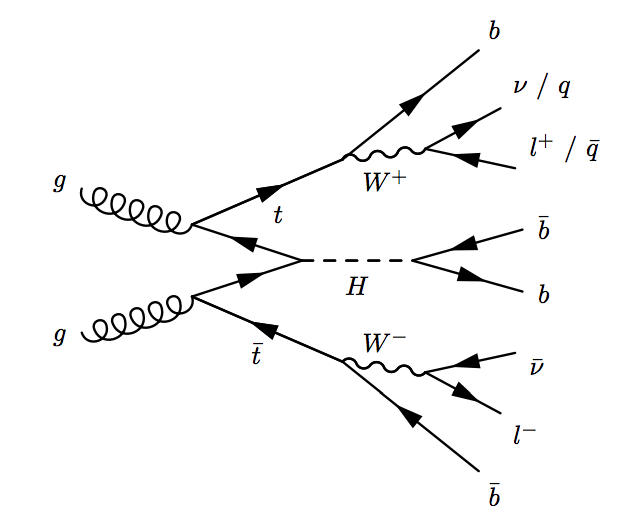
\includegraphics[scale=0.3]{imgs/ttH_feynman.png}
		\caption{Feynman diagram of the \ttbar and Higgs boson production.}
		\label{fig:ttH}
	\end{center}
\end{figure}

Neutrinos ($v\bar{v}$) do not interact with the detector, so their characteristics are not recorded. Since the top quark reconstruction requires the neutrinos information, their characteristics are analytically determined with the remaining data, known as kinematical reconstruction. However, the \ttbar system may not have a possible reconstruction: the reconstruction has an intrinsic uncertainty associated which determines its accuracy.

\begin{figure}[!htp]
	\begin{center}
		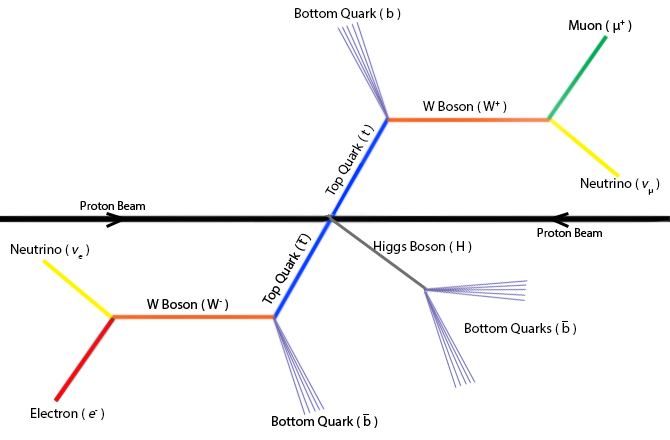
\includegraphics[scale=0.45]{imgs/ttbar_higgs.png}
		\caption{Schematic representation of the \ttbar system and Higgs boson decay.}
		\label{fig:ttbar}
	\end{center}
\end{figure}

The amount of jets from bottom quarks and leptons present in the events may vary according to the decay channel of the $W$ bosons produced in the top quark decays. As shown in figure \ref{fig:ttbar}, four jets and two leptons are required to be present in the events. Two of the jets and two leptons are needed to reconstruct the \ttbar system, and the remaining two jets are used for the Higgs boson reconstruction. For the kinematical reconstruction, every possible combination of jets and leptons must be evaluated and only the most accurate reconstruction is considered. If the $t\bar{t}$ system has a possible solution, the Higgs boson is reconstructed from the jets of the two remaining bottom quarks. The Higgs reconstruction does not use the jets that were associated to the best \ttbar system reconstruction. The overall quality of the event processing depends on the combined accuracy of both reconstructions.

For the global event reconstruction, several solutions can be tested if we assume that the ATLAS detector has an experimental energy-momentum resolution of $\pm1\%$, by varying these quantities within their uncertainty. This uncertainty is propagated into the \ttbar system and Higgs analysis, affecting their accuracy. To improve the quality of the reconstructions several random variations are applied to the measured values, within a maximum range of $|1\%|$ next to the measured values, and apply the process explained previously for each variation. The quality of the event analysis and the application execution time is directly proportional to the amount of variations performed. The goal is to do as many variations as possible within a reasonable time frame.

The current version of \tth, the application developed to perform this analysis, is capable of reconstructing \~3000 events per second on a 2.60 GHz \intel Xeon CPU, without the accuracy improvement. Physicists consider that 1000 variations within the $\pm1\%$ uncertainty would have a big impact on the analysis accuracy, but for \tth is only capable of processing 5 events per second with this precision. The reconstruction of the \ttH system accounts for 99.8\% of \tth execution time with this level of accuracy. To be viable to analyse the \ttH system with 1000 variations it is crucial to improve the \tth efficiency.

\section{Goals and Scientific Contribution}
\label{goals}

Dealing with scientific applications developed by scientists is not trivial due to the code structure and organisation. Several studies \cite{SC:Nature,SC:Develop,SC:SC11,SC:28280} identified the causes that lead scientists to produce poor code:

\begin{center}
	\begin{itemize}
		\item Most scientists are self-taught programmers with inadequate or outdated computer science background.
		\item Scientists disregard software engineering principles to produce efficient code that is also robust, modular, and long lasting.
		\item Scientists often iteratively develop over the same application, producing legacy code (some applications currently in production are iterated on for the last 20 years), and not documenting it so that it can be used by others.
		\item Scientists are seldom aware of profiling and debugging tools, as well as parallelization paradigms.
		\item Scientists cannot afford to get into the architectural details of the newer generations of computing systems, reducing the portability of the code they produce.
	\end{itemize}
\end{center}

To improve the quality of the scientific code, scientists agree that it is crucial to create an interface between their field and computer science by having multidisciplinary teams. However, computer scientists often lack the expert field specific knowledge required to be acknowledged as an integral part of these teams. This often makes scientists sceptical to let others restructure, and even develop from scratch, legacy code that they have been using for years.

The goal of this PhD dissertation is to provide an efficient unified framework for the development of particle physics data analysis applications, designed in close cooperation with the LIP research group. It aims to give an abstraction to the current data analysis programming model, so that the user only codes the sections relative to each specific data analysis, while the framework guarantees portable efficiency for both homogeneous and heterogeneous platforms. The physics researchers will spend less time developing applications, while the framework ensures that the code is automatic parallelized and efficiently uses the computing power of both CPUs and accelerator devices, improving both the data analysis accuracy and throughput.

With a more agile development of high performance data analysis applications, researchers can spend more time improving the algorithms accuracy, which also require the extra computing power provided by the efficient use of multicore CPUs and manycore devices, and analysing larger amounts of data. These two factors have a significant impact on improving the quality of the physics research.

The specialised design of the framework for the specific field of particle physics data analysis allows to implement better automatic parallelization mechanisms than the equivalent general purpose frameworks. On homogeneous platforms, it has been demonstrated in \cite{paperAMP,Msc:AMP} that a single shared or distributed memory parallel implementation may not provide the best efficiency when compared to an hybrid implementation. This framework will attempt to use hybrid parallel configurations in specific cases on a single computing system, while other frameworks assume that shared memory paradigm best suits all applications needs. On heterogeneous platforms, the framework will initially support automatic parallelization for both \nvidia GPU and \intel Xeon Phi devices, with dynamic load balance among CPU and accelerator devices. The framework will use an efficient load balance library for heterogeneous platforms (most libraries only support GPUs), and possible extend its performance model to support the use of \intel Xeon Phi hardware accelerators.

\section{Document Structure}
\label{structure}

This document is structured as follows:

\begin{description}
	\item[Introduction:] this chapter contextualises the work in section \ref{context}, and presents the scientific problem that motivates the PhD thesis proposal in section \ref{motivation}. Section \ref{goals} presents the goals and scientific contribution of this PhD.
	\item[State of the Art:] this chapter presents the current hardware and software technology available for homogeneous and heterogeneous platforms in sections \ref{homo_systems} and \ref{hetero_systems}, respectively. Section \ref{particle_frameworks} contextualises the current work on data analysis optimisation and available libraries for particle physics. Section \ref{tools} presents the available tools and libraries to profile parallel applications.
	\item[An Unified Particle Physics Framework:] the current particle physics skeleton library used by the LIP research group is presented in section \ref{lipminianalysis}. Section \ref{new_framework} presents the conceptual design and preliminary prototypes of the efficient particle physics framework proposed for the PhD thesis.
	\item[Research Plan:] the research plan for the PhD thesis work is presented in this chapter.
\end{description}

%!TEX root = ../main.tex

\chapter{State of the Art}
\label{state_of_the_art}

\section{Hardware}
\label{hardware}

Computing clusters are a common resource among scientific research groups. These massively parallel systems are usually constituted by racks of computing nodes interconnect by a specialised network, but each running an individual instance of the operating system. The cluster operates on a distributed memory configuration, where shared data must be explicitly transferred among nodes. These cluster nodes may be different but use a common interface to communicate with each other.

Clusters use dedicated nodes to centralise the data storage and implement an abstraction layer to the user. When running an application, the user file system is mounted on the nodes that will perform the computation, but it is still needed to manually copy all necessary data to avoid unnecessary communication. The computing nodes architecture may be homogeneous or heterogeneous.

\subsection{Homogeneous Systems}
\label{homo_systems}

Homogeneous systems are the most common computing platforms, constituted by one or more CPU devices with their own memory bank (RAM memory), and are interconnected by a specific interface. Although these systems use a shared memory model, where all the data is addressable among multiple CPUs, each CPU has its own physical memory bank, which causes the system to have a Non Unified Memory Access (NUMA) pattern, as presented in figure \ref{fig:homoplat}. This means that the access time of a CPU to a piece of memory in its memory bank will be faster than accesses to the other CPU bank. The threads of an application must have the data that they will use on the memory bank of their CPU device to avoid the increased communication costs of NUMA.

\begin{figure}[!htp]
	\begin{center}
		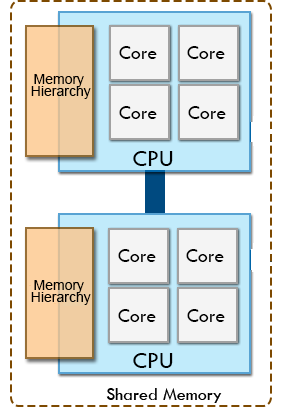
\includegraphics[scale=0.45]{imgs/homoplats.png}
		\caption{Schematic representation of a homogeneous system.}
		\label{fig:homoplat}
	\end{center}
\end{figure}

\subsubsection*{CPU devices}
\label{cpu_devices}

Gordon Moore predicted, in 1965, that for the following ten years the number of transistors on the CPU chips would double every 1.5 years \cite{MooreLaw}. This was later known as the Moore’s Law and it is expected to remain valid at least up to 2015. Initially, this allowed the increase in CPU chips clock frequency by the same factor as the transistors. Software developers did not spend much effort optimising their applications and only relied on the hardware improvements to make them faster.

The clock frequencies of CPU chips started to stall in 2005 due to thermal dissipation issues. Manufacturers shifted from making CPUs faster to increasing their throughput by adding more cores to a single chip, reducing their energy consumption and operating temperature. This marked the beginning of the multicore and parallel computing era, where every new generation of CPUs get wider, while their clock frequencies remain steady.

CPU devices are designed as general purpose computing units, and may contain multiple cores, each based on a simple structure of small processing units attached to a very fast hierarchical memory (cache, whose purpose is to hide the high latency access to global memory), and all the necessary data load/store and control units. They are capable of delivering a good performance in a wide range of operations, from executing simple integer arithmetic to complex branching and SIMD (single instruction multiple data, later explained) instructions. A single CPU core implements various mechanisms for improving the performance of applications, at the hardware level, with the most important explained next:

\begin{center}
	\begin{description}
		\item[ILP] instruction level parallelism (ILP) is the overlapping of instructions, performed at both the hardware and software level, which otherwise would run sequentially. At the software level, ILP is implemented as static parallelism, as compilers try to identify which instructions are data independent, meaning that the outcome of one does not affect the execution of the other, and schedules them to execute simultaneously, if the hardware has resources to do so. At the hardware level, ILP can be referred as dynamic parallelism, since the hardware dynamically identifies which instructions execution can be overlapped while the application is running.

		\item[Vector instructions] are a special instruction set based on the SIMD model, where a single instruction is simultaneously applied to a large set of data. CPUs offer special registers to allow executing an operation on a chunk of data in a special arithmetic unit. One of the most common examples is addition of two vectors, where the hardware is capable of adding a given number of elements simultaneously . This optimisation is often performed at compile time.

		\item[Multithreading] is the hardware support for the execution of multiple threads in a CPU core. This is possible by replicating part of the CPU resources, such as registers, and can lead to a more efficient utilisation of the CPU core hardware. If one thread is waiting for data, other thread can resume execution while the former is stalled. It also allows a better usage of resources that would otherwise be idle during the execution of a single thread. If multiple threads are working on the same data, multithreading can reduce the synchronisation costs between them, as they both operate on the same CPU core, and may lead to a better cache usage.
	\end{description}
\end{center}

\subsection{Heterogeneous Systems}
\label{hetero_systems}

A new type of computing platform is becoming increasingly popular, with the emergence of specialised hardware designed to efficiently solve a specific set of computing problems. This marks the beginning of heterogeneous systems, where one or more CPU devices operate in a shared memory environment as in homogeneous systems, presented in subsection \ref{homo_systems}, and are coupled with one or more hardware accelerators. CPUs and accelerators operate in a distributed memory environment, meaning that data must be explicitly passed between the CPU and the accelerator by the programmer.

\begin{figure}[!htp]
	\begin{center}
		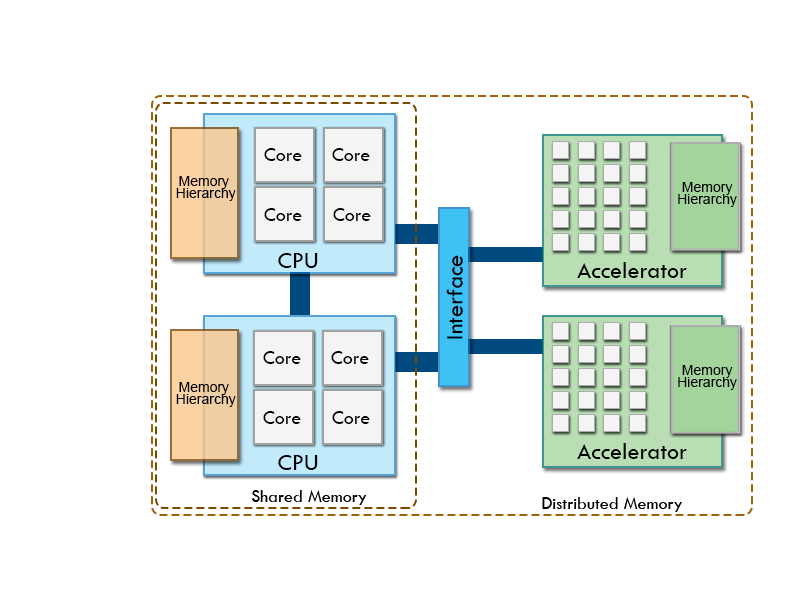
\includegraphics[scale=0.45]{imgs/heteroplats.png}
		\caption{Schematic representation of a heterogeneous system.}
		\label{fig:heteroplat}
	\end{center}
\end{figure}

Figure \ref{fig:heteroplat} presents a schematic representation of a heterogeneous system. Both CPUs use the same interface to communicate with the hardware accelerators, which may cause contention in the communications to between devices. This high latency PCI-Express interface is usually a potential bottleneck for applications that use hardware accelerators.

Computing accelerators are usually constituted of a large number of small and simple processing units, aimed to achieve the most performance possible on specific massively parallel problems, as opposed to general purpose CPUs. This massive data parallel processing (SIMD execution model) offered by these accelerators, where a single operation is performed simultaneously on large quantities of independent data, have the purpose of offloading the CPU from such data intensive operations. Several manycore accelerator devices are currently available, with me most popular being the general purpose GPUs and Intel Many Integrated Core line, with its production device known as Intel Xeon Phi \cite{Intel:MIC}. An heterogeneous platform may have one or more accelerator devices of the same or different architectures.

As of June 2014, 62 of the TOP500’s list \cite{TOP500} are computing clusters that use hardware accelerators, which indicates an exponential growth of these devices popularity compared to previous years. The Intel Xeon Phi is becoming increasingly popular, being the accelerator device of choice in 17 clusters of the TOP500, with 2 of those clusters on the top 10 (the fastest cluster, Tianhe-2, uses this device). NVidia GPUs remain as the most used accelerator, on a total of 44 clusters with 2 on the top 10, but the AMD devices are steadily losing their share. The most popular hardware accelerators will be presented in depth in the next subsections.

\subsubsection*{Graphics Processing Unit}
\label{gpu}

The Graphics Processing Units (GPU) were one of the first hardware accelerators on the market. Their initial purpose was to accelerate computer graphics applications, which started of as simple pixel drawing and evolved to support complex 3D scene rendering, such as transforms, lighting, rasterisation, texturing, depth testing, and display. Due to the industry demand for customisable shaders, this hardware later allowed some flexibility for the programmers to modify the image synthesising process. This also allowed using this GPUs as a hardware accelerator for wider purposes beyond computer graphics, such as scientific computing, as some researchers saw the potential to use these devices to boost the performance of numerical computation.

The GPU architecture is based on the SIMD execution model. Image synthesising is, from the computational point of view, the processing of a large set of numbers that represent pixels. The processing of each individual pixel usually does not depend on the processing of its neighbours, or any other pixel on the image, so, in the best case scenario, the computation has no data dependencies, which allows to process all pixels simultaneously. The massive data parallelism is the most important characteristic that was considered when designing the GPU architecture.

As GPU manufacturers allowed more flexibility to program their devices, the High Performance Computing (HPC) community started to use these devices to solve specific massively data parallel problems, such as numerical computation problems. However, the highly specialised architecture of GPUs affected the performance of many other different problem domains. Due to the increased demand for these devices by the HPC community, manufacturers began to generalise more of the GPUs features, such as adding support for double precision floating point arithmetic, and later began producing accelerators specifically oriented for scientific computing. \nvidia is the main GPU manufacturer for scientific computing GPUs, with a wide range of available hardware known as Tesla. These devices characteristics differ from the general purpose GPUs, as they have more GDDR RAM, a different structural design to fit in cluster nodes, and different cooling options. The chip itself is different, offering more processing units and larger memory caches. Kepler \cite{NVIDIA:Kepler} is the latest GPU architecture released by \nvidia, and its relevant design details are explained next.

\begin{figure}[!htp]
	\begin{center}
		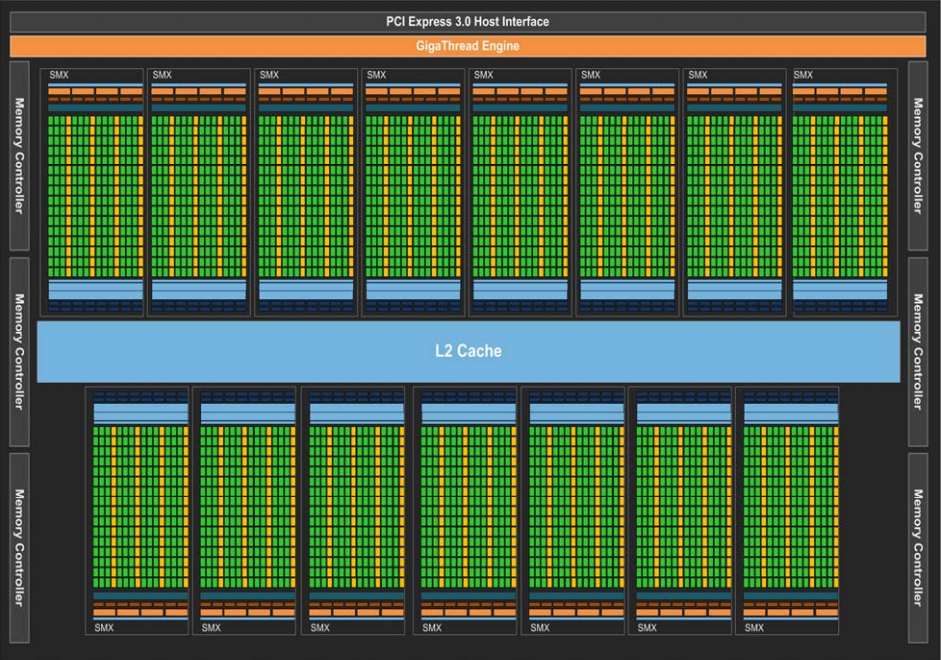
\includegraphics[scale=0.45]{imgs/kepler_arch.png}
		\caption{Schematic representation of the \nvidia Kepler architecture.}
		\label{fig:kepler}
	\end{center}
\end{figure}

Figure \ref{fig:kepler} shows the Kepler architecture organisation in two main components: the Streaming Multiprocessor (SMX) and the memory module. The focus of this architecture was not only on improving the performance but also the energy efficiency, offering up to to 3x more performance per watt than Fermi (the previous architecture). To achieve this efficiency, Kepler has implemented several features to improve the computational resource usage:

\begin{description}
	\item[Dynamic Parallelism:] a kernel (algorithm coded in CUDA) running on the GPU is capable of calling itself recursively, which allows to dynamically generate new workload to process without the CPU interference. This improves irregular algorithms performance on the GPU and reduces the communications to the CPU as the GPU is capable of managing the workload.
	\item[Hyper-Q:] this technology increases the amount of work queues to 32 simultaneously hardware managed connections. It allows for multiple CPU cores to launch different kernels on the GPU simultaneously, improving the device resource usage. Multiple threads of the same application are able to share the GPU resources, reducing the amount of synchronisations.
	\item[Grid Management Unit:] to allow for dynamic parallelism a new grid (a collection of threads of a kernel, explained in more detail in subsection \ref{distributed_mem}) management system is required. The new system also allows to schedule multiple grids simultaneously, which allows for different kernels, from possibly different threads, to run concurrently (Hyper-Q).
	\item[\nvidia GPUDirect:] this feature allows GPUs in a single system, or in a interconnected network, to share data without the interference of the CPU and system memory, creating a direct connection to Solid State Drives and other similar devices, reducing the communication latency.
\end{description}

The SMX are complex processing units responsible for performing all computations on the GPU, and there may be up to 15 in a single chip. Each SMX has 192 single precision and 64 double precision CUDA cores, small processing units capable of performing basic arithmetic, 32 special function units, to perform complex computations such as trigonometric operations, and 32 load and store units. These computing units operate at the GPU main clock rate. The SMX features 4 warp schedulers (warps are presented in subsection \ref{distributed_mem}) and 8 instruction dispatchers.

Each SMX has 65536 32-bit registers, with a maximum of 255 registers per CUDA thread, a 64 KByte very fast memory for L1 cache and shared memory, and a similar fast 48 KByte memory cache for read-only data. Finally, the Kepler architecture provides 1536 KB of L2 cache shared among all SMX units. The high end available Tesla K40 has a memory bandwidth of 280 GB/s to its main memory. Since the GPU is connected by PCI-Express interface, the bandwidth for communications between CPU and GPU is restricted to only 12 GB/s (6 GB/s in each direction of the channel). Memory transfers between the CPU and GPU must be minimal as they may greatly restrict the performance.

A kernel is executed by a given amount of parallel workers named CUDA threads. They are grouped into blocks, to be scheduled among SMX and the threads inside a block can only run in a given SMX, and these are grouped into a grid, which contains all CUDA threads (up to $2^{31}-1$) for a given kernel. The CUDA threads are grouped in batches of 32, called warps, to be dispatched by a warp scheduler. The scheduler has a scoreboard with up to 48 entries to manage which warps are stalled waiting for resources or data and which are ready to be executed.

\subsubsection*{Intel Many Integrated Core architecture}
\label{mic}

The \intel Many Integrated Core (MIC) architecture, with the current production device being the \intel Xeon Phi, is an emerging technology adopted by various clusters in the TOP500 list. It has a design different from the \nvidia GPUs presented previously, opting to have fewer computing units but capable of performing more complex operations, and heavily relying on code vectorisation to extract performance. Figure \ref{fig:mic} presents a schematic representation of the architecture. The current high end model, the \intel Xeon Phi 7120p, has 61 cores and 16 GB GDDR5 RAM. The device has three operating modes:

\begin{description}
	\item[Native:] the device acts as an independent system itself, with one core reserved for the operating system execution. The application and all libraries must be compiled specifically to run on the device, and later copied to the its memory along with the necessary input data, prior to its execution. No further interaction with the CPU is required until the application has executed.
	\item[Offload:] the device acts an accelerator, such as a GPU. Only part of the application is set to run on the Xeon Phi, and data required by the code must be explicitly passed between CPU and the device. All library functions called inside the device must be specifically compiled for it.
	\item[Message passing:] the device acts as an individual computing system in the network. Memory transfers are explicitly and the device can be programmed using the Message Passing Interface (MPI) \cite{MPI}. The restrictions mentioned in the previous point are also applicable.
\end{description}

\begin{figure}[!htp]
	\begin{center}
		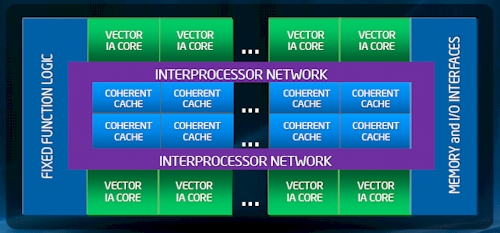
\includegraphics[scale=0.65]{imgs/mic.png}
		\caption{Schematic representation of the \intel Many Integrated Core architecture.}
		\label{fig:mic}
	\end{center}
\end{figure}

Each core is able to run 4 threads simultaneously, and most of the massive parallelism is obtained by using the vectorisation capabilities provided by the 32 512 bit wide vector registers available. However, only a small set of vector operations are implemented in the hardware, and the most complex are emulated by the compiler. Each core as 64 KB for data and 64 KB for instruction L1 cache, and 512 KB L2 cache. There is no shared cache among the 61 cores of the chip, and no cache consistency and coherence is automatically guaranteed among them. The cores are interconnected by a bidirectional ring network. MIC does not support out of order execution, which greatly compromises the use of ILP. Also, the clock frequency is limited to 1.1 GHz, which is less than half of the modern CPUs.

Since it uses the same instruction set as conventional x86 CPUs, \intel claims that current applications can be easily ported to run on the device. This may be true for common matrix arithmetic and similar applications, efficient ports of complex applications that require the use of many external libraries is very difficult, or even infeasible \cite{Msc:AMP}.

The next iteration of the MIC architecture, known as Knights Landing, will provide out of order execution, better branch prediction, and implement all AVX vector operations in hardware, as in current \intel CPUs. It will also use a new instruction set, more similar to x86, to allow an easier port of most C++ features to the device.

\subsubsection*{Other hardware accelerators}
\label{other_accelerators}

Many alternative hardware accelerators are currently on the market due to the increasingly popularity of GPUs and Intel MIC among the HPC community. Texas Instruments developed their new line of Digital Signal Processors, best suited for general purpose computing while very power efficient. Their capable of delivering 500 GFlop/s (giga floating point operations per second), consuming only 50 Watts \cite{Texas:DSP}.

ARM processors are now leading the mobile industry and, alongside the new NVidia Tegra processors \cite{NVIDIA:Tegra} that are steadily increasing the market share, are likely to be adopted by the HPC community\footnote{e.g. the ARM based Montblanc project will replace the MareNostrum in the Barcelona Supercomputing Center (BSC)} due to their low power consumption while delivering a significant performance \cite{ARM}. Due to the increased complexity of mobile applications, the shift from 32 bit to 64 bit mobile processors has already happened, which will greatly benefit computing clusters using this type of hardware.

\section{Software}
\label{software}

Both computer scientists and self-taught programmers are only used to code and design sequential applications, showing a lack of know-how to develop algorithms for parallel environments. This lack of expertise is even more evident when programming for heterogeneous systems, where programming paradigms shift among different hardware accelerators. The mainstream industry is still adopting the use of multicore architectures with the purpose of increasing their processing performance, which reflects in a lack of academic training of computer scientists on code optimisation and parallel programming. Self taught programmers have an increased obstacle due to the lack of theoretical basis when using these new parallel programming paradigms.

Programming for multicore environments requires some knowledge of the underlying architectural concepts of CPU devices and how they are interconnected. Shared memory, cache coherence and consistency, and data races are architecture-specific aspects that the programmer does not face in sequential execution environments. However, these concepts are fundamental not only to efficiently use the computational resources, but to ensure the correctness of applications.

Heterogeneous systems combine the flexibility of multicore CPUs with the specific capabilities of manycore accelerator devices. However, most computational algorithms and applications are designed to the specific characteristics of CPUs. Even multithreaded applications cannot be easily ported to these devices expecting high performance. To optimise the code it is necessary a deep understanding of the architectural principles behind these devices design.

The workload balance between the cores of a single CPU chip is an important aspect to extract performance and get the most efficient usage of the available resources. A inadequate workload distribution may cause some cores of the CPU to be starved, unnecessarily increasing the application execution time. A good load balancing strategy ensures that all the cores are used as much as possible. Considering a multi-CPU system, it is important to manage the data in such a way that it is available in the memory bank of the CPU that will need it to avoid the increased NUMA latency. The same concepts apply when balancing the load between CPU and hardware accelerators, with the increased complexity of the distributed memory environment and high latency data transfers.

Some computer science groups developed libraries that attempt to abstract the programmer from specific architectural and implementation details of these systems, providing an easy API as similar as possible to current sequential programming paradigms. The next subsections will present frameworks to aid the development of parallel applications for homogeneous and heterogeneous systems, frameworks used in particle physics, and tools to profile and identify bottlenecks in parallel code.

\subsection{Shared Memory Environments}
\label{shared_mem}

Homogeneous systems often operate in a shared memory environment. Using multiple CPU devices may cause the memory banks to be physically divided but hardware mechanisms, such as specialised CPU interconnections, allow for a common addressing space. Libraries and frameworks for parallelizing for this environment are presented next.

\subsubsection*{pThreads}

Threads are the most simple parallel task that can be scheduled by the operating system. POSIX Threads (pThreads) are the standard implementation for UNIX based operating systems with POSIX conformity, such as most Linux distributions and Mac OS. The pThreads API provides the user with primitive for thread management and synchronisation. Since this API forces the user to deal with several low level implementation details, such as data races and deadlocks, the industry demanded the development of high abstraction level libraries, which are usually based on pThreads.

\subsubsection*{OpenMP, TBB, and Cilk}

OpenMP \cite{OpenMP}, Intel Threading Building Blocks (TBB) \cite{Intel:TBB}, and Cilk \cite{Intel:Cilk} are the most popular high level libraries for parallel programming in homogeneous systems.

The OpenMP API is designed for multi-platform shared memory parallel programming in C, C++, and Fortran, for most CPU architectures available. It is portable and scalable, and aims to provide a simple and flexible interface for developing parallel applications, even for the most inexperienced programmers. It is based in a work sharing strategy, where a master thread spawns a set of slave threads and compute a task in a shared data structure.

Intel TBB employs a work stealing heuristic, where, after the initial load distribution, if the task queue is empty, a thread attempts to steal a task from other busy threads. It provides a scalable parallel programming task based library for C++, independent from architectural details, and only requires a \intel C++ compiler. It automatically manages the load balancing and some cache optimisations, while offering parallel constructors and synchronisation primitives for the programmer. However, it requires knowledge of the object oriented programming paradigm.

Cilk is a runtime system for multithreaded programming in C++. It maintains a stack with the remaining work, employing a work stealing heuristic similar to the Intel TBB.

\subsection{Distributed Memory Environments}
\label{distributed_mem}

Heterogeneous systems use distributed memory address space for handling the data between CPU and accelerator devices. Even though the CPU devices work on a shared memory space, data must be explicitly passed to the accelerators. General purpose frameworks for parallelizing on the devices and on the heterogeneous platforms as a whole are presented next.

\subsubsection*{Message Passing Interface}

The Message Passing Interface (MPI) \cite{MPI}, designed by a consortium of both academic and industry researchers, has the objective of providing a simple API for process based parallel programming in distributed memory environments. It relies on point-to-point and group messaging communication, and is available in Fortran and C. It is often used in conjunction with a shared memory parallel programming API, such as OpenMP, for work sharing among computing nodes, with the latter ensuring a more efficient parallelization inside each node.

Intel adapted an MPI version to work across their CPUs and Xeon Phi, considering the device as an individual computing node. Communications between the CPU and the device are explicitly handled by the programmer by calling specific functions. The other alternative to program for this device with MPI is to use compiler \textit{pragma} directives for data communication and code parallelization.

\subsubsection*{CUDA}

The Compute Unified Device Architecture (CUDA) is a computing model for hardware accelerators launched in 2007 by \nvidia and aims to provide a framework for programming devices similar architecture to the \nvidia GPUs. It has a specific instruction set architecture (ISA) and allows programmers to use GPUs for scientific computing.

\nvidia considers that a parallel task is constituted by a set of CUDA threads, which execute the same instructions coded in the kernel but on different data. For instance, in the sum of two vectors each CUDA thread will be responsible for adding a single element of the vectors.

The CUDA thread is the most basic data independent parallel task, which can run simultaneously with other CUDA threads, and it is organised in a hierarchy presented in figure \ref{fig:cuda}. A block is a set of CUDA threads that is matched to a specific SMX by the global scheduler. The thread blocks are organised in a grid, which represents the whole parallel tasks of a kernel. Note that both the blocks and the grid sizes must be defined by the programmer, according to the algorithm, before calling the kernel, within the maximum values allowed by the GPU architecture. A warp is a subset of CUDA threads from a block that are set to run simultaneously on a SMX.

\begin{figure}[!htp]
	\begin{center}
		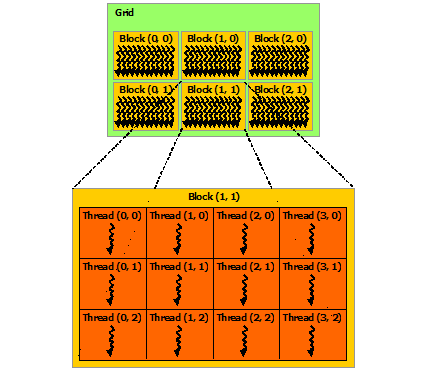
\includegraphics[scale=0.9]{imgs/cuda_threads.png}
		\caption{Schematic representation of CUDA thread hierarchy.}
		\label{fig:cuda}
	\end{center}
\end{figure}

Conditional jumps are a special type of instructions that must be avoided as they cause different CUDA threads within the same warp to diverge. Since an SMX does not allow threads to execute different instructions simultaneously, the divergent branches will execute sequentially, doubling the warp execution time.

\subsubsection*{DICE}

The DICE framework aims to provide the tools to help building efficient and scalable applications for heterogeneous platforms with accelerator devices that support CUDA. It creates an abstraction layer between the architectural details of heterogeneous platforms and the programmer, aiding the development of scalable parallel applications. Its main focus is to obtain the best performance possible on irregular applications, rather than abstracting all the architecture details from the programmer. It is still required to the programmer to have some knowledge of each different architecture and respective programming paradigms, and the framework needs to be instructed of how tasks should be divided in order to fit the requirements of the different devices. 

Instead of relying in pre-partitioned work, the programmer defines a function for dicing the dataset and the framework creates different sized chunks of data to distribute among the CPU and GPUs. The framework frees the programmer from managing the workload distribution, memory usage and data transfers among the available devices, but requires that the application is built according to its strict specifications. The programmer is able to tune specific details related to the memory transfers and load balance, if he has the required expertise with the framework.

The scheduler uses the statistics provided by each job (a kernel set to run on a device) to adjust the scheduling policy and the granularity of the tasks. This dynamic granularity management allows to better suit the uneven execution times of irregular jobs. DICE uses a variant of the Heterogeneous Earliest Finish Time (HEFT) scheduling algorithm \cite{HEFT}, which uses the computation and communication costs of each task, in order to assign every task to a device in such a way that minimises the estimated finish time of the overall task pool. This variant of HEFT attempts to make a decision every time it is applied to the task pool, so that tasks on the multiple devices take the shortest possible time to execute \cite{Msc:Mariano}.

DICE assumes a hierarchy composed of multiple devices (both CPUs and GPUs, in its terminology), where each device has access to a private address space (shared within that device), and a distributed memory system among devices. To abstract this distributed memory model, the framework offers a global address space. However, since the communication between different devices is expensive, DICE uses a relaxed memory consistency model, where the programmer can use a synchronisation primitive to enforce memory consistency. DICE implements a shared software cache so that every device has the data as close as possible, using the local memory of each device. It also ensures that each device has a copy of a given data partition, which otherwise would only be stored in the CPU memory.

\subsubsection*{StarPU}

StarPU \cite{STARPU} is a unified runtime system consisting on both compiler directives and a runtime API that aims to allow programmers to efficiently extract parallelism from heterogeneous platforms by abstracting the architecture details of these systems. This framework frees the programmer of the workload scheduling and data consistency inherent from the distributed memory environment of heterogeneous platforms. Task submissions are handled by the StarPU task scheduler, and data consistency is ensured via a data management library.

However, one of the main differences to DICE is that StarPU attempts to increase performance by carefully considering and attempting to reduce memory transfer costs. This is done using history information for each task and, accordingly to the scheduler decision of where a task shall be executed, as it asynchronously deals with data dependencies while the system is busy computing the tasks that are ready. The task scheduler can take this into account, and determine where a task should be executed by considering not only the execution history, but also the estimation of data transfers latency.

StarPU employs a task based approach to the programming model, where a kernel is considered a parallel task. Based on the scheduler and available implementations for the kernel (i.e., can only run on CPU, GPU, or both), the framework handles where and how much load each task will compute. It provides a set of different schedulers for the programmer to chose.

The performance model differs among the schedulers implemented in StarPU, but most track the tasks execution time on the devices. All the schedulers use a user defined calibration to start the execution, and after 10 executions of each task it starts to perform a real-time calibration with the available statistics. This may translate in an inefficient usage of the system resources at the start of the application, but ensures that it tends to improve as the application runs.

The memory consistency is automatically ensured by the framework, as it transfers the data asynchronously without the programmer interaction. The data dependencies are determined by the scheduler, with some interaction of the programmer, when declaring if a data structure is read/write or both. The granularity of the tasks must be defined by the user, as opposed to the DICE dynamic adjustment.

\subsubsection*{OpenACC}

OpenACC \cite{OpenACC} is a framework for heterogeneous platforms with accelerator devices. It is designed to simplify the programming paradigm for CPU/GPU systems by abstracting the memory management, kernel creation, and GPU management. Like OpenMP, it is designed for C, C++ and Fortran, it provides both an API and compiler directives, and allows the parallel task to run on both CPU and GPU at the same time. However, it does not schedule the load between the CPU and GPU, as it is only designed to offload the workload to the accelerators. The current specification addresses both \nvidia and AMD GPUs, as well as the \intel Xeon Phi.

This framework focus on creating an abstraction of the hardware accelerator used, focusing on portability across heterogeneous platforms, rather than abstracting the intrinsic complexities of these systems.

\subsubsection*{OpenHMPP}

OpenHMPP \cite{OpenHMPP} is a standard similar to OpenACC, designed by CAPS \cite{CAPS} to develop parallel applications for heterogeneous platforms. It attempts to abstract the complexities of GPU accelerators by providing a set of compiler directives for efficient parallelization. In the current specification, OpenHMPP uses a superset of the OpenACC directives for offloading code to the GPU and managing the data transfers, in both C and Fortran.

Although it provides asynchronous execution of the offloaded kernel, it is not possible to use this framework to manage simultaneous execution and load balance of the same kernel in both CPUs and GPUs. Moreover, it is only possible to use this specification with the CAPS compilers and PathScale ENZO Compiler Suite \cite{ENZO}.

\subsection{Particle Physics Frameworks}
\label{particle_frameworks}

\subsubsection*{ROOT}

ROOT \cite{CERN:ROOT} is a complex framework designed by particle physicists to aid all data analysis application development of the physics experiments conducted at CERN. It has all functionality required to process large amounts of data, by providing specific data storage formats, C++ classes for elemental particles, various physics algorithms, and histogram creation functions. The framework also provides a built-in C++ interpreter, Cling, to allow testing simple instructions and macros, without the need to compile and link the code.

PROOF is a subset of the framework to support the development of data analysis applications in distributed memory environments. However, it is only designed to work with a set of computing nodes, on a master/slave process hierarchy, without the support for hardware accelerators. Also, it does not focus on the efficient usage of the available computational resources, as it only distributes the load on demand among the processes.

Currently, ROOT does not provide any features parallelized, but the developers already shown interest to improve the performance of some of the core routines of the framework by parallelizing them on a shared memory environment. However, it may not translate in massive performance gains of the data analysis applications, as their critical regions are usually the reconstruction of the events, which do not rely on those complex ROOT functionalities, but rather on a large set of simple routines and classes.

\subsubsection*{TopROOTCore}

TopROOTCore is an extension of ROOT for top quark physics, developed by CERN associate research groups, which adds features and physics algorithms to the existing framework. It is responsible for producing the last input data format at the last CERN computational tiers, before the final analysis and event reconstruction. In the data analysis applications, it is often used due to some physics algorithms it implements.

\subsection{Profiling Tools and Libraries}
\label{tools}

\subsubsection*{Performance API}

The Performance API (PAPI) \cite{PAPI} specifies an API to access hardware performance counters in most modern processors. It allows programmers to measure the performance counters for specific regions of an application, evaluating metrics such as cache misses, operational intensity or even power consumption. This analysis helps classifying the algorithms and identify possible bottlenecks at a very low abstraction level.

PAPI recently supports hardware counters for both \nvidia GPUs, using the \nvidia CUPTI driver interface, and \intel Xeon Phi. It also supports counters to measure the energy efficiency of the hardware.

\subsubsection*{\nvidia CUPTI}

The \nvidia CUDA Profiling Tools Interface (CUPTI) \cite{NVIDIA:CUPTI} is a performance analysis interface available in the \nvidia drivers for CUDA capable GPUs. It provides a callback API to integrate with the code, at the entry and exit of a kernel call, which monitors the interaction of the code with the CUDA runtime and drivers. CUPTI has a second API to monitor the performance of a kernel on the GPU by analysing the hardware counters on the device, which allows for a in-depth assessment of the code behaviour in memory transactions, cache accesses and misses, and much more.

\subsubsection*{TAU and HPCToolkit}

TAU \cite{TAU} and HPCToolkit \cite{HPCToolkit} are performance analysis tools, with static and dynamic functionalities, to evaluate the performance of HPC applications. The static APIs are low level and, while providing higher control of the areas to profile and specific metrics, require the programmer a deeper knowledge of these tools and how to integrate them with the existing code. The dynamic functionalities provide general metrics but do not require any changes to the application code.

Both tools provide statistical visualisation GUIs, to build graphs and comparisons of the different metrics profiled during the application execution time. Note that both tools support the analysis of parallel code in shared and distributed memory environments, but the HPCToolkit still does not support hardware accelerators. Unlike VTune, these tools only present the statistics but do not attempt to identify the bottlenecks, leaving that task to the programmer.

\subsubsection*{VTune}

Intel VTune profiler \cite{Intel:VTune} is a proprietary tool for performance analysis of parallel applications. It provides an easy to use interface to analyse applications, automatically identifying its bottlenecks, without requiring any change to the source code. It intercepts the system calls to assess the execution time and behaviour, such as efficient cache usage, of the routines of an application. VTune also provides visualisation functionalities to make the profiling of parallel applications a simple task for developers with small experience. It works with both \intel and GNU compilers.

\subsubsection*{VampirTrace}

VmpirTrace \cite{VampirTrace} is a open source library to analyse an application execution on both shared and distributed memory environments, with support for CUDA capable GPUs through the CUPTI driver interface. It is capable of analysing the CPU hardware counters per thread/process by resorting to the Performance API. It has a low level API to integrate with the code to measure specific metrics and regions of the code, and a more abstract interface that allows tracing the application execution without the need to change the code.

Additionally, VampirTrace allows to analyse the I/O interactions of an application, such as access times, types, and patterns to the hard drives.

\subsubsection*{\nvidia Nsight}

The \nvidia Nsight \cite{NVIDIA:Nsight} is a development platform for heterogeneous computing. It is available for both Visual Studio and Eclipse and aids the development of code for CUDA capable GPUs, with easy integration with current official production libraries. It has real time debugging functionalities to test code running on both CPU and GPU simultaneously. The built-in profiler allows to perform analysis to the kernels execution time on GPU, load and store efficiency (related to the coalesced accesses of CUDA threads to memory), SMX occupancy rate, and memory usage. The profiling metrics are the same as the ones provided by the Performance API, as they both use the \nvidia CUPTI interface.

%!TEX root = ../main.tex
\chapter{An Unified Efficient Particle Physics Framework}
\label{new_lipmini}

Programming for homogeneous platforms poses a series of challenges not faced when coding parallel applications due to the shared memory paradigm. In this context, the data is always easily accessible when coding, as the different memory bank accesses are managed by the compiler and hardware. Data dependencies and races still need to be managed by the programmer, which may required a significant level of expertise. To efficiently use the computational resources, dealing with problems such as false sharing or efficient cache usage, the programmer must have an advanced expertise on both the coding and architectural details of homogeneous platforms.

Since an heterogeneous platform is a distributed memory environment, where the CPUs shared the memory with each other but not with the hardware accelerators, a series of new challenges arise. All communications of data between CPU and accelerator must be explicitly coded by the programmer, and has an added latency associated. The balance of the work for each computing device to process becomes harder as it must take into account the data transfers and different characteristics of the devices.

Each different hardware accelerator has its own architectural design principles, as show in section \ref{hardware}, which constrain the way they are programmed and the characteristics that both the algorithm and the code must have to efficiently use the computational resources. This implies that the programmer must be able to learn the hardware intrinsic characteristics and adapt to a new programming paradigm. Even for experienced programmers, adapting current applications to run on heterogeneous platforms may be infeasible without redesigning all major algorithms, as opposed to code a new application specifically for these platforms. This issue has an higher impact on legacy code.

Scientists are usually self-taught programmers that only consider coding as a necessary tool to perform their research. Several studies, referred in section \ref{motivation}, identified a set of problems with scientists coding practices and scientific computing. Most of their code is in constant development, up to decades long, only adding or changing functionalities in each iteration, not considering any software engineering principles and not adapting the code to the changes in hardware. The few that worry about performance attempt to address the code regions that they think are the bottleneck, not knowing of the existence of profiling tools and even compiler optimisations.

Since most scientists develop applications with the help of specialised frameworks of their research field, they expect them to be efficient, by resorting to parallelisation or other techniques. However, the bottleneck is often on the scientists code rather than in the framework, and these tools are not designed to automatically extract parallelism from their code.

Scientists usually do not have any training for programming efficient applications for homogeneous systems or cluster environments, as programming is just a necessity for their field of research. They are even more reluctant to learn the new programming paradigms required to work with hardware accelerators on heterogeneous platforms. With this in mind, several automatically parallelisation frameworks for these systems were developed by computer scientists, as presented in subsection \ref{distributed_mem}.

These general purpose frameworks usually have a steep learning curve, even for computer scientists. One significant setback of these frameworks is that, even if it is not explicitly required, the application must be designed to the framework characteristics, rather than the framework adapt to the application. As scientists are usually reluctant to redesign the very complex legacy code, which is difficult for computer scientists to understand without the expertise of the science field, an integration with these frameworks is infeasible. This problem also applies to the most of the external libraries used by these applications, as their functions are not coded to run on hardware accelerators and adapting the source code may not be possible.

Even though, scientists are not willing to endure the steep learning curve of these frameworks to integrate with future applications, and do not want to code two versions of the core algorithms to run on the CPU and accelerator. Their complexity and the lack of guarantees to that they will increase the code performance, due to poor implementation or algorithm characteristics, puts the scientists further away from these frameworks. Also, they attempt to have few dependencies of an application with external libraries, as the external tools are not guaranteed to be supported through the application lifetime.

The existence of general purpose automatically parallelisation frameworks is useful, specially for computer scientists, but the scientific community lacks frameworks that both address the intrinsics of their scientific field, in which scientists can trust and rely, and the efficient usage of the computational resources, on both homogeneous and heterogeneous platforms. Frameworks such as these sacrifice the abstraction to interact with any scientific field, but are more adapted to the scientific problem that is addressed. A lower abstraction level leads to an easy interaction of the scientist with the tool (and even abstract them of any parallelisation complexities) and increases the computational efficiency of the code when compared with general purpose frameworks, as the main bottlenecks are usually known \textit{a priori} and the framework is designed around their characteristics. The development of such frameworks may lead to a better interface of computer scientists and researchers, causing and improvement of their codes with the implementation of software engineering concept, increasing the quality of the research.

\section{The LipMiniAnalysis Skeleton Library}
\label{lipminianalysis}

The LipCbrAnalysis was a skeleton developed by two researchers of LIP in 2005, with the purpose of aiding the development of data analysis applications within the research group. Initially it served as an interface for dealing with the I/O of the data, transforming it from the format supported by ROOT at the time to variables in the global memory of the skeleton. All other standard functions needed for the analysis had their prototypes declared, but it was the programmers job to code them to his needs, knowing that the required data for each event was on memory.

Along the years the code was successively iterated to add support for new data file formats, physics functionalities, and general features, such as the support for passing options and arguments to the executable. Some of the functions that the programmer needed to code were now fully implemented, with the option of being override by the user.

The LipMiniAnalysis is the latest development iteration on a production environment. It discarded outdated features that were no longer necessary, and reads the new Mini Ntuple data format, hence its name. It is not a standard ROOT data format, but rather a set of events that suffered some preprocessing to improve the quality of the data and filter events that do not show any interesting physics.

Figure \ref{fig:lipmini} presents the structure of LipMiniAnalysis, where all sections marked with a \textbf{*} need to be coded by the programmer. When the application starts it sets the default values for all control information needed by the event filtering and reconstruction. The \textit{Set User Values} section allows for the user to set its own control parameters, for both information defined by \textit{Set Default Values}, overwriting the existing configuration, and parameters not set yet. The \textit{Get Command Line Options} section is responsible for defining and interpreting the options defined by the user when starting the executable. It is partially defined with standard options for every analysis, such as the definition of the systematics file and output directory, but the programmer can add new options as needed. The systematics parameters are automatically configured based on the input systematics file, so no user interaction is necessary. The preparation of both the input and output files is done automatically, but the declaration of the histogram vectors must be coded by the programmer, as it depends on the event type, filtering and reconstruction techniques applied.

\begin{figure}[!htp]
	\begin{center}
		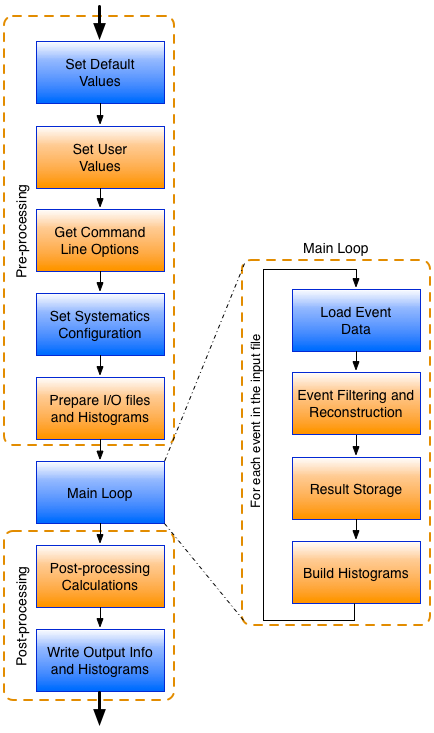
\includegraphics[scale=0.5]{imgs/lipminianalysis.png}
		\caption{Schematic representation of the LipMiniAnalysis skeleton structure. The \textbf{*} mark represents the sections of the skeleton that the programmer must code.}
		\label{fig:lipmini}
	\end{center}
\end{figure}

The \textit{Main Loop} is responsible for individually loading an event from the input file, apply the filters, reconstruct it if it passes the required filters, store the results, and build the histograms for each filter and final reconstruction. Only the event loading is automatic, so the programmer must code all remaining sections, as they vary among different analysis. The final post-processing also depends on the analysis, so it is not coded. Then, LipMiniAnalysis automatically writes all output information. Note that this is a logical structure of the code; in the current implementation most features are not properly organised and LipMiniAnalysis would have great benefits from a reorganisation of its structure, code-wise.

Studies presented in \cite{Msc:AMP,paperAMP} targeted the computational efficiency issues of a specific data analysis application of LIP, related to the reconstruction of the \ttH system. This data analysis was developed using the LipMiniAnalysis and, although the goal was to address only the inefficiencies of the data analysis itself, problems with the main data structure of the skeleton restricted the performance scalability, specially on heterogeneous platforms.

The LipMiniAnalysis was designed to store only one event in the application global memory for the \textit{Main Loop} to load and process. The data for an event is composed of hundreds of variables, from simple scalars to complex vectors of ROOT classes. With only a single event in memory, it is more difficult to create an efficient parallelisation with only the event reconstruction tasks, due to the low amount of work to balance, specially on distributed memory environments as it will require more communications through the application lifetime. With all events from an input data file on the application global memory, a more efficient parallelisation for both shared and distributed memory systems can be achieved. It would also help the implementation of automatic parallelisation in LipMiniAnalysis.

\section{The Proposed Framework}
\label{new_framework}

A physics framework to replace LipMiniAnalysis in aiding the development of data analysis applications is proposed. Its design and specification will include several software engineering concepts to provide a stable and robust tool that will increase the researchers productivity, spending less time coding and more time analysing data and improving physics algorithms, and ensure the generation of efficient data analysis applications by automatically parallelising the code. It will include both redesigned features of LipMiniAnalysis and new physics functionalities.

Improving both the researcher coding productivity and data analysis computational efficiency has a direct impact on the research quality. To achieve this goal, the proposed framework has to utilise the capabilities of modern computing systems and software. This implies that the LipMiniAnalysis code design, based on the LipCbrAnalysis developed in 2005, does not suit the characteristics of current hardware. The new framework will implement all required features present in LipMiniAnalysis but designed to modern specifications of hardware, software, and modularity to interact with new features.

Figure \ref{fig:new_framework} presents the organisation and dependencies of the different modules of the proposed framework. A modular organisation and implementation allows for the framework to be robust and easily extensible in the future. The \textit{Physics} and \textit{Histograming} modules will be implemented using redesigned features currently available at LipMiniAnalysis, as they have standard features used by most data analysis applications. The framework will have to support both ROOT and TopROOTCore libraries without any specific configuration by the user. TopROOTCore installation with the framework may be an option to the user, since only a part of event data analysis applications use its functionalities, which are more useful for data preparation.

\begin{figure}[!htp]
	\begin{center}
		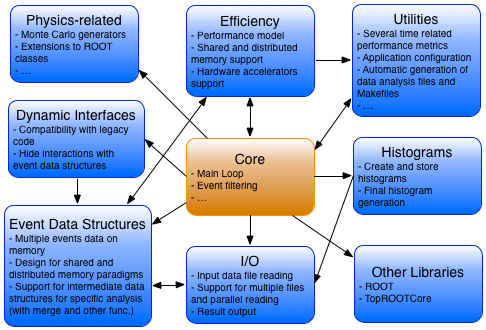
\includegraphics[scale=0.7]{imgs/new_framework.png}
		\caption{Schematic representation of the proposed framework modules and their dependencies.}
		\label{fig:new_framework}
	\end{center}
\end{figure}

The \textit{I/O} module is responsible for loading the input data files for processing the events in the data analysis applications. The LipMiniAnalysis reads only MiniNtuples, which are preprocessed events at the previous computational tiers, which are used by some applications, but other file formats may also be supported, as requested by researchers. Different file formats have different structures and auxiliary event parameters stored, although the core event information is similar. The file reading must support parallel file descriptors, so that it is possible that each thread/process reads its own event data, reducing the communications cost and initial load distribution overhead.

The \textit{Event Data Structures} module will be dependent on the file type to be read. Its purpose is to have a C++ class, or set of classes, to hold all the information of an event on memory in a structured way, opposed to the current implementation on LipMiniAnalysis. Then, it must hold a STL collection (vector, map, etc) to store the instantiations of the event class, enclosing all events in the input data file. An assessment of the different file formats used at LIP will be required to evaluated the benefits of having a single abstract event class or specific classes for each file format. Both the event class design and storing collection must be suitable for both shared and distributed memory parallelisation, with good performance for data structure splits (to balance the load, specifically in distributed memory paradigms), transverses (to iterate through the events on each split segment), and low overhead (un)marshalling computations for communicating the data. The module may also contain specific data structures for intermediate processing, as explained in detail in subsection \ref{work_so_far}, suitable to run on hardware accelerators, considering the limitations that they incur.

The \textit{Dynamic Interfaces} module will hold the interface generator and respective interfaces for each different event data structure. Its purpose is to make the framework compatible with legacy code, allowing for current data analysis to benefit from the automatic parallelisation and improved efficiency of the proposed framework. Also, it must hide the interaction of the user with the data structures, to provide a simpler programming interface, later explained in more detail. Since there may be several different data structures, and their code may be changed periodically, the interface generator must be capable of parsing the data structure source files and dynamically generate the interfaces.

The \textit{Utilities} module implements several auxiliary features usable in both the framework and data analysis code. It will have simple performance statistics, such as execution time of the application, communications time, event processing throughput, etc. A more robust command line options reader will be available, with all required options for executing all different data analysis, which can be extended by experienced users.

The \textit{Efficiency} module will have all necessary functionality required to create parallel tasks and manage the load distribution for both homogeneous and heterogeneous platforms with hardware accelerators. The performance model must be capable of assessing if an hybrid multithreaded process parallelisation provides better efficiency than a simple implementation, which was proven to happen in some data analysis \cite{paperAMP}. There is no automatic parallelisation tool that attempts hybrid implementations such as this, only opting for a shared or distributed memory paradigm (usually the last is only used when the hardware forces to) and uses an efficient amount of parallel tasks, but it may prove beneficial to have this mix of processes and threads in some specific cases. This might require an higher overhead to obtain the best process/thread configuration, but since these data analysis run for several hours the initial setup cost is minimum. It also can produce a configuration file when the configuration is performed for a given data analysis on a given computing system, which can avoid performing the initial setup every time the application is executed.

This module must also be able to assess, with some help of the user, what sections of the data analysis code can be executed in the hardware accelerators, and if it has the required characteristics to efficiently use these devices. While this might seem complex for general purpose parallelisation frameworks, dealing with only a specific problem such as physics data analysis applications helps the design of the performance model around these features. Implementation-wise, these features require heavy modifications to current automatic parallelisation frameworks. However, a new implementation designed to this specific problem, with components adapted from current frameworks, may provide a better and more simple integration and performance efficiency of data analysis applications.

The \textit{Core} module will integrate all previous modules, implementing the major routines responsible for the event analysis, ranging from the filtering to the final output data storage. It will have assembled all the specific bits of each module to process the events, as well as the code sections that is for the user to code. Note that the user will not edit the code in the framework, but rather on the data analysis source code that will later link the missing parts into the framework.

Features that are very important for the most compute intensive sections of data analysis applications will be implemented to run on CPU and accelerator devices. These features will be provided in the framework API. For example, when selecting an pseudo-random number generator to use in a compute intensive section, such as the event reconstruction, the user must avoid the \texttt{TRandom} available in ROOT and use the one provided by the framework. The framework compiles the code to run on CPU, which uses \texttt{TRandom}, and on GPU, which uses the \texttt{cuRand} (with the same PRNG algorithm). This only applies for features that produce the same result on any computing accelerator. Otherwise, an alternative is suggested for each computing device that the user may chose to accept.

\subsection{Usage and Workflow}
\label{usage_workflow}

One of the goals of the framework is to provide a kernel-like programming model to the user, with as minimum interaction as possible. This eases the development of new data analysis applications and increases their portability. Once the framework is installed on a system, the user just needs to copy their code and it is expected to compile, as all external dependencies are handled by the framework. Its flow is presented in figure \ref{fig:new_framework_flow}. Note that LipMiniAnalysis, presented in section \ref{lipminianalysis}, has a similar logical structure, but it does not reflect the code organisation and structure. In the new framework, the code will follow this structure to improve its modularity and reliability.

\begin{figure}[!htp]
	\begin{center}
		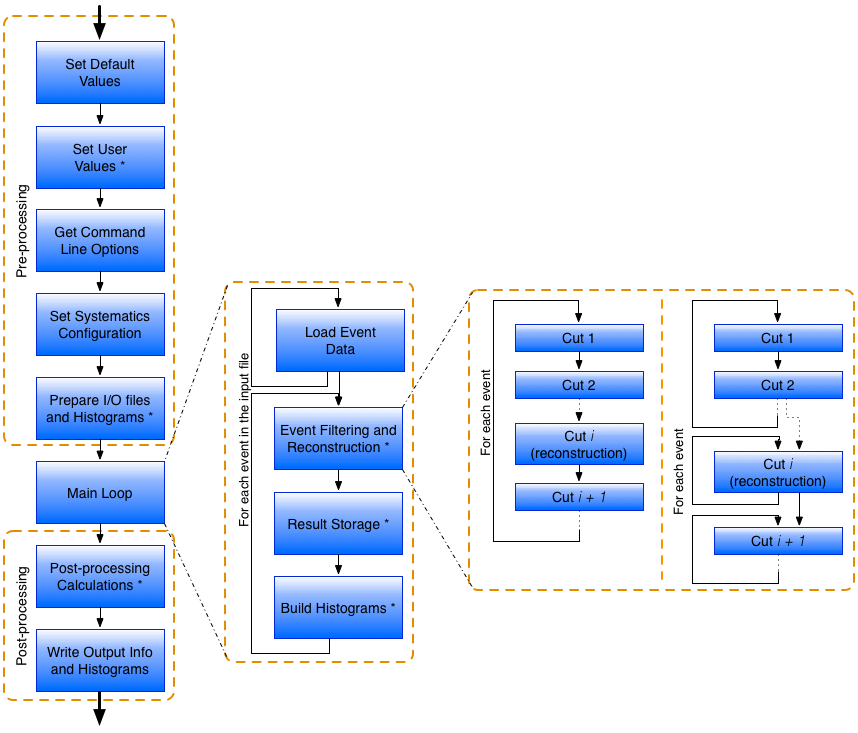
\includegraphics[scale=0.5]{imgs/new_framework_flow.png}
		\caption{Schematic representation of the proposed framework flow. The \textbf{*} mark represents the sections of the workflow coded by the programmer.}
		\label{fig:new_framework_flow}
	\end{center}
\end{figure}

The user intervention is required at four stages of the event processing (implementation-wise, the \textit{Result Storage} and \textit{Build Histograms} are coded together as \textit{Filter Post-process}). The data analysis is expected to be implemented as a class, which will extend the \texttt{DataAnalysis} class provided by the framework, and must contain at least a set of predefined methods that represent each of the stages that the user must code. The coding is very intuitive, as the user must implement the set of features required to process a single event, in the logical pipeline reasoning. The user does not interact directly with the event data structure, but through the respective interface, which gives the illusion that only a single event is on memory, as physicists were used to program. The framework will be responsible for applying the code in parallel to all events on memory, not necessarily following the pipeline order but respecting the dependencies.

The data analysis stages are characterised as follows:

\begin{description}
	\item[\textit{User Setup}:] this is only executed at the beginning of the data analysis execution, where the user specifies the initial \textit{User Values}, as in the LipMiniAnalysis flow, output files, and histogram configurations. The user can also easily specify any additional parameters to read by both command line and environment variables, using the respective framework utilities, and a small set of configurations to help the parallelisation setup.
	\item[\textit{Event Filtering and Reconstruction}:] this holds the code required to filter and reconstruct a single event. As shown in figure \ref{fig:new_framework_flow}, two templates are provided. The first is the traditional pipeline for the event processing, oriented for novice users. The second provides three sections: pre-filtering, reconstruction, and post-filtering. The user codes in the pre-filtering the filters applied before the reconstruction, the reconstruction, and then the final filters (if applicable), in three separate methods. This is useful when the reconstruction takes most of the execution time and this provides more parallelism (as it is applied simultaneously to all events) and better load management, specially when using heterogeneous platforms.
	\item[\textit{Result Storage} and \textit{Build Histograms}:] this is coded as a single method, since both operations are closely dependent in most implementations. The user store the results of the previous filtering to later be printed in the output file.
	\item[\textit{Post-processing Calculations}:] this stage is executed once, after processing all events. The user codes all final calculations before the results and histograms output.
\end{description}

Note that this design of the stages required by the \texttt{DataAnalysis} class will be changed after the requirements elicitation and an usability study with the LIP researchers. All major features are initial design and testing is performed in close cooperation with a subset of LIP physicists, working on top quark and Higgs boson research.

However, the programmer will have some guidelines to avoid producing an inefficient data analysis. Class variables in \texttt{DataAnalysis} must be avoided because of the amount of communications required to maintain the consistency and coherence of that data on a distributed memory environment. To maintain portability, the data analysis must only depend on the libraries provided by the framework (at the moment, there is none data analysis in LIP that depends on other libraries). To run on heterogeneous platforms, the analysis critical region must only depend on features that the framework has implemented for both CPU and accelerator devices. This allow for the user to code the data analysis once and the critical regions are able to execute on any computing device. Otherwise, the code will be restricted to the device that can execute it.

\subsection{Preliminary Prototypes}
\label{work_so_far}

Some of the work towards the creation of the new framework was already developed. These prototypes were integrated and tested with the current version of LipMiniAnalysis using the \ttH data analysis application presented in \ref{ttH}, but have a modular design to be properly merged into the final framework, and they may suffer structure or implementation changes throughout its development. Proposed prototypes for several features required by the framework are presented next.

\subsubsection*{A new event data structure}

The information of an event is loaded in the \textit{Main Loop} into a single global memory state. The hundreds of variables of an event are spread among a set of files of LipMiniAnalysis. To create a new event data structure all these variables must be merged into a single C++ class, which represents a single event, named \textit{EventData}, and use a standard collection, such as a STL vector, to store all events on an input file. However, the current LipMiniAnalysis version performs a set of data preparation routines, named \textit{FillAllVectors} and \textit{Calculations}, performed automatically and coded by the user, respectively. As their implementation is only prepared to access the data as it was in the global memory, they will not be compatible with the new data structure. 

The implementation of \textit{Calculations} could be changed in order to access the values stored in the new data structure. However, the user would have to be aware of the data structure interaction and characteristics to properly code the required data preparation. Also, since \textit{Calculations} only access the data of an event, it makes much more sense to code it as a method of the event class. The current implementation of \textit{EventData}, the \textit{FillAllVectors} routine, which performs the initialisation of some of the components of an event, is coded as a method, and the \textit{Calculations} is declared as a virtual function, so it can be easily coed by the user in the analysis source file, without the need of modifying the LipMiniAnalysis code and recompile the skeleton.

\subsubsection*{A new \textit{Main Loop} design}

Having a new data structure that allows multiple events to be on memory simultaneously implies changes to the way that LipMiniAnalysis handles the input data files. Instead of loading an event at a time, the \textit{Main Loop} implementation was changed to load all events in an input data file at once and store them in the new specialised structure (note that an input file has a size of 1 GBytes), as presented in figure \ref{fig:new_loop}. Now, it is possible to parallelise the execution of the \textit{Event Filtering and Reconstruction}, performed in the \textit{DoCuts} function. In physics terminology, a filter is addressed as a cut.

\begin{figure}[!htp]
	\begin{center}
		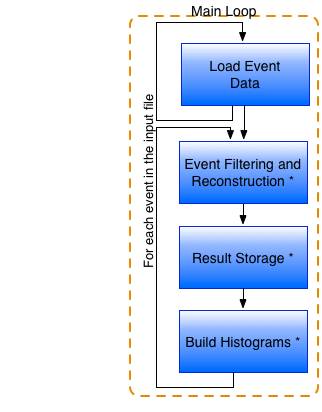
\includegraphics[scale=0.5]{imgs/new_loop.png}
		\caption{Schematic representation of the \textit{Main Loop} implementation modifications.}
		\label{fig:new_loop}
	\end{center}
\end{figure}

The interaction of the LipMiniAnalysis with the input data file is performed using the ROOT file reader classes. Since the event loading assumes also a set of operations, such as storing MonteCarlo information on \textit{EventData} and the \textit{FillAllVectors} initialisation, this task would benefit if it was executed in parallel, as the I/O itself only amounts to part of the computation. However, up to version ROOT v6, released in early June, it was not possible to have parallel file descriptors reading information of the same input file. With the new ROOT version it may be possible but it was not yet tested.

As previously stated, the \textit{DoCuts} function is responsible for filtering and reconstructing the events. The purpose of these filters is to separate the signal (interesting events) from the background (uninteresting events). The notion of an interesting event depends on the physics that the analysis studies, for example the background of a \ttH system analysis may contain events useful for the search of heavy quarks. As it may vary among different analysis, the \textit{DoCuts} must be coded by the user, but its structure is well defined. Implementation-wise, an analysis has a set of filters. Each filter is logically composed by a set of computations, more or less complex, and a test to the results of those computations. If the test fails, the event is not submitted to the rest of the filters. An example of a simple filter is to check if the mass of the event system (aggregate masses of all or a subset of particles detected) is greater than a given value, discarding events that do not provide interesting physics.

The reconstruction of an event is considered as a filter in \textit{DoCuts}, as only the events capable of being reconstructed pass the filter, which is usually the last. The reconstruction may be the most complex and computational intensive task in the whole data analysis application. One example is the \ttH system reconstruction, which performance depends on a trade-off between reconstruction accuracy and execution time. The event reconstruction is a task that may require a closer look to improve the efficiency of the data analysis, through a more specialised parallelisation on both homogeneous and heterogeneous platforms. Its irregular load and execution time, very complex algorithms, and few vectorised numerical computations creates a bottleneck complex to deal with, but with the potential of bringing exceptional performance gains when addressed with detail \cite{paperAMP}. Figure \ref{fig:new_docuts} presents a implemented prototype for a new \textit{DoCuts} flow that exposes the event reconstruction to more efficient parallelism approaches.

\begin{figure}[!htp]
	\begin{center}
		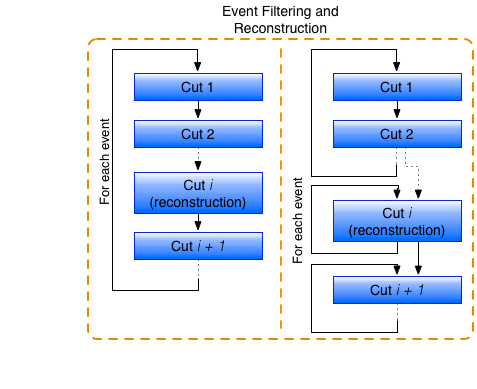
\includegraphics[scale=0.5]{imgs/new_docuts.png}
		\caption{Schematic representation current (left image) and proposed (right image) \textit{Event Filtering and Reconstruction} flows.}
		\label{fig:new_docuts}
	\end{center}
\end{figure}


Besides exposing the parallelism of a complex computational intensity section, this change also increases the workload to be simultaneously processed. When the application reaches the reconstruction, all events that passed the previous cuts can be processed in parallel. Having all the data necessary outside of the \textit{Main Loop}, as the \textit{Event Filtering and Reconstruction} as its own loop over all events on memory, but still hiding that fact from the user that codes \textit{DoCuts} to abstract the user as explained in \ref{new_framework}, allows for a better load balance of the possible parallelisation approaches, for homogeneous and heterogeneous platforms. For the latter, which operate in a distributed memory environment, it also helps to reduce the parallelisation overhead associated with the communications: instead of passing required the data of a single event multiple times, the data of all events is passed once. Then there is a third section of cuts (post-reconstruction) that are also coded by the user. To reduce the amount of loops, this third section shares the loop over all events with all the remaining post-processing of the \textit{Main Loop}. Note that both \textit{Main Loop} options will be available to maintain compatibility with the current data analysis applications.

\subsubsection*{Interfacing with legacy code}

Current data analysis use the data of an event as it is on the global memory, with no structure. The integration of the new event data structure requires that the accesses to the data be made through the STL collection used to store the event and the \textit{EventData} class. An interface is proposed to avoid rewriting the legacy code of these data analysis, a way to abstract the user from programming for a set of events by providing a kernel-like approach (where the code for processing an event is automatically applied to all). The interface must abstract both the access to the \textit{EventData} variables and methods, while being completely transparent to the user.

The input data files occasionally suffer some changes do to the increase in information given by the previous preprocessing on the CERN computational tiers. The file reading and the \textit{EventData} classes have to be adapted to this increase in event parameters. A static interface would need to be rewritten every time such change occurred. To avoid this problem, a parser was developed that receives the \textit{EventData} source files and retrieve the name of the methods and parameters. It then creates an header composed of \textit{define} clauses that translate the accesses to these variables on the STL collection to the previous simple accesses. This header is then included in the main LipMiniAnalysis header so that the user does not need to interact with the interface. This interface is automatically created every time the skeleton is compiled.

The user can code the data analysis assuming a single event is stored in memory. For example, to access an event luminosity the user would write \texttt{int var = LumiBlock}. However, when compiling the application the compiler preprocessor uses the interface to replace that statement with \texttt{int var = events.get(currentEvent).getLumiBlock()} without the user knowing how the event is stored. Note that the counter that assigns the event to process is automatically managed in every loop that iterates through the event data structure, hidden from the user.

\subsubsection*{Other features}

The final framework will have an utilities module where general features will be coded. Some of the already implemented range from automatic execution time measurement of the application and event processing throughput, definition of the number threads to execute, set the accuracy of some reconstructions. It was opted to use environment variables to set these features to reduce the clutter of options currently passed to the data analysis applications (usually more than 10 parameters) and separate general purpose features from physics functionalities.

One complex feature implemented is specific for the \ttH data analysis application. During the event reconstruction, several different variations of the system are reconstructed and only the best is of interest. For that a class was developed that encloses the resultant data of the reconstruction and performs a parallel merge through all the threads. This feature might prove useful for other data analysis once the structure of the class is general enough to hold the result of different types of reconstructions.

%!TEX root = ../main.tex
\chapter{Research Plan}
\label{thesis_planning}

The research plan for the PhD thesis work is organised as follows:

\begin{itemize}
	\item For the first semester of 2014/2015:
	\begin{itemize}
		\item Requirements elicitation of all physics features to implement on the framework together with the LIP researchers.
		\item Validate the proposed framework design and new data analysis programming model.
		\item Redesign of the features already implemented in LipMiniAnalysis to fit the new framework requirements.
		\item Assess and compare the performance of various C++ collections to store various events on memory.
		\item Extend the current event data structure to fit the requirements of all data analysis:
		\begin{itemize}
			\item By adding the all variables in the ROOT input data files, or;
			\item By the user defining which variables are needed for a given analysis, and the data structure being automatically created using that information;
		\end{itemize}
		\item Extend the I/O features available in LipMiniAnalysis:
		\begin{itemize}
			\item By reading multiple input data files in parallel;
			\item By build the event data structure in parallel;
		\end{itemize}
		\item Assess and compare the performance of DICE, StarPU, and Legion libraries and their available performance models for irregular workload balance in:
		\begin{itemize}
			\item Homogeneous systems;
			\item Heterogeneous systems with hardware accelerators;
			\item Heterogeneous cluster nodes;
		\end{itemize}
		\item Support for hybrid process/thread automatic parallelization with partial integration with the chosen parallelization library.
	\end{itemize}
	\item Present the first framework prototype without hardware accelerator support in March 2015.
	\item For the second semester of 2014/2015:
	\begin{itemize}
		\item Assess the extendibility of the chosen parallelization framework to support the \intel Xeon Phi hardware accelerator.
		\item Complete the proposed framework integration with the parallelization library to support GPU accelerators.
		\item Adapt the parallelization library to support \intel Xeon Phi accelerator.
	\end{itemize}
	\item For 2015/2016:
	\begin{itemize}
		\item Update the state of the art research on software and hardware environments for heterogeneous platforms.
		\item Improve the performance across multiple computing nodes in cluster environments.
		\item Extend the functionalities of the proposed framework.
		\item Thesis write up.
	\end{itemize}
\end{itemize}



%\bibliographystyle{../../common/IEEE}
%\nocite{*}
\newpage % force the bookmark to go to the new page
\pdfbookmark{References}{references}
\printbibliography[title=References]

%\input{tex/910_signatures}

\end{document}
